% Options for packages loaded elsewhere
\PassOptionsToPackage{unicode}{hyperref}
\PassOptionsToPackage{hyphens}{url}
%
\documentclass[
]{article}
\usepackage{amsmath,amssymb}
\usepackage{iftex}
\ifPDFTeX
  \usepackage[T1]{fontenc}
  \usepackage[utf8]{inputenc}
  \usepackage{textcomp} % provide euro and other symbols
\else % if luatex or xetex
  \usepackage{unicode-math} % this also loads fontspec
  \defaultfontfeatures{Scale=MatchLowercase}
  \defaultfontfeatures[\rmfamily]{Ligatures=TeX,Scale=1}
\fi
\usepackage{lmodern}
\ifPDFTeX\else
  % xetex/luatex font selection
\fi
% Use upquote if available, for straight quotes in verbatim environments
\IfFileExists{upquote.sty}{\usepackage{upquote}}{}
\IfFileExists{microtype.sty}{% use microtype if available
  \usepackage[]{microtype}
  \UseMicrotypeSet[protrusion]{basicmath} % disable protrusion for tt fonts
}{}
\makeatletter
\@ifundefined{KOMAClassName}{% if non-KOMA class
  \IfFileExists{parskip.sty}{%
    \usepackage{parskip}
  }{% else
    \setlength{\parindent}{0pt}
    \setlength{\parskip}{6pt plus 2pt minus 1pt}}
}{% if KOMA class
  \KOMAoptions{parskip=half}}
\makeatother
\usepackage{xcolor}
\usepackage[margin=1in]{geometry}
\usepackage{color}
\usepackage{fancyvrb}
\newcommand{\VerbBar}{|}
\newcommand{\VERB}{\Verb[commandchars=\\\{\}]}
\DefineVerbatimEnvironment{Highlighting}{Verbatim}{commandchars=\\\{\}}
% Add ',fontsize=\small' for more characters per line
\usepackage{framed}
\definecolor{shadecolor}{RGB}{248,248,248}
\newenvironment{Shaded}{\begin{snugshade}}{\end{snugshade}}
\newcommand{\AlertTok}[1]{\textcolor[rgb]{0.94,0.16,0.16}{#1}}
\newcommand{\AnnotationTok}[1]{\textcolor[rgb]{0.56,0.35,0.01}{\textbf{\textit{#1}}}}
\newcommand{\AttributeTok}[1]{\textcolor[rgb]{0.13,0.29,0.53}{#1}}
\newcommand{\BaseNTok}[1]{\textcolor[rgb]{0.00,0.00,0.81}{#1}}
\newcommand{\BuiltInTok}[1]{#1}
\newcommand{\CharTok}[1]{\textcolor[rgb]{0.31,0.60,0.02}{#1}}
\newcommand{\CommentTok}[1]{\textcolor[rgb]{0.56,0.35,0.01}{\textit{#1}}}
\newcommand{\CommentVarTok}[1]{\textcolor[rgb]{0.56,0.35,0.01}{\textbf{\textit{#1}}}}
\newcommand{\ConstantTok}[1]{\textcolor[rgb]{0.56,0.35,0.01}{#1}}
\newcommand{\ControlFlowTok}[1]{\textcolor[rgb]{0.13,0.29,0.53}{\textbf{#1}}}
\newcommand{\DataTypeTok}[1]{\textcolor[rgb]{0.13,0.29,0.53}{#1}}
\newcommand{\DecValTok}[1]{\textcolor[rgb]{0.00,0.00,0.81}{#1}}
\newcommand{\DocumentationTok}[1]{\textcolor[rgb]{0.56,0.35,0.01}{\textbf{\textit{#1}}}}
\newcommand{\ErrorTok}[1]{\textcolor[rgb]{0.64,0.00,0.00}{\textbf{#1}}}
\newcommand{\ExtensionTok}[1]{#1}
\newcommand{\FloatTok}[1]{\textcolor[rgb]{0.00,0.00,0.81}{#1}}
\newcommand{\FunctionTok}[1]{\textcolor[rgb]{0.13,0.29,0.53}{\textbf{#1}}}
\newcommand{\ImportTok}[1]{#1}
\newcommand{\InformationTok}[1]{\textcolor[rgb]{0.56,0.35,0.01}{\textbf{\textit{#1}}}}
\newcommand{\KeywordTok}[1]{\textcolor[rgb]{0.13,0.29,0.53}{\textbf{#1}}}
\newcommand{\NormalTok}[1]{#1}
\newcommand{\OperatorTok}[1]{\textcolor[rgb]{0.81,0.36,0.00}{\textbf{#1}}}
\newcommand{\OtherTok}[1]{\textcolor[rgb]{0.56,0.35,0.01}{#1}}
\newcommand{\PreprocessorTok}[1]{\textcolor[rgb]{0.56,0.35,0.01}{\textit{#1}}}
\newcommand{\RegionMarkerTok}[1]{#1}
\newcommand{\SpecialCharTok}[1]{\textcolor[rgb]{0.81,0.36,0.00}{\textbf{#1}}}
\newcommand{\SpecialStringTok}[1]{\textcolor[rgb]{0.31,0.60,0.02}{#1}}
\newcommand{\StringTok}[1]{\textcolor[rgb]{0.31,0.60,0.02}{#1}}
\newcommand{\VariableTok}[1]{\textcolor[rgb]{0.00,0.00,0.00}{#1}}
\newcommand{\VerbatimStringTok}[1]{\textcolor[rgb]{0.31,0.60,0.02}{#1}}
\newcommand{\WarningTok}[1]{\textcolor[rgb]{0.56,0.35,0.01}{\textbf{\textit{#1}}}}
\usepackage{graphicx}
\makeatletter
\def\maxwidth{\ifdim\Gin@nat@width>\linewidth\linewidth\else\Gin@nat@width\fi}
\def\maxheight{\ifdim\Gin@nat@height>\textheight\textheight\else\Gin@nat@height\fi}
\makeatother
% Scale images if necessary, so that they will not overflow the page
% margins by default, and it is still possible to overwrite the defaults
% using explicit options in \includegraphics[width, height, ...]{}
\setkeys{Gin}{width=\maxwidth,height=\maxheight,keepaspectratio}
% Set default figure placement to htbp
\makeatletter
\def\fps@figure{htbp}
\makeatother
\setlength{\emergencystretch}{3em} % prevent overfull lines
\providecommand{\tightlist}{%
  \setlength{\itemsep}{0pt}\setlength{\parskip}{0pt}}
\setcounter{secnumdepth}{-\maxdimen} % remove section numbering
\usepackage{hyperref}
\hypersetup{colorlinks=true, linkcolor=red, urlcolor=blue}
\ifLuaTeX
  \usepackage{selnolig}  % disable illegal ligatures
\fi
\IfFileExists{bookmark.sty}{\usepackage{bookmark}}{\usepackage{hyperref}}
\IfFileExists{xurl.sty}{\usepackage{xurl}}{} % add URL line breaks if available
\urlstyle{same}
\hypersetup{
  pdftitle={(Fast) Introduction to R - Class 2},
  pdfauthor={Joana Cima},
  hidelinks,
  pdfcreator={LaTeX via pandoc}}

\title{(Fast) Introduction to R - Class 2}
\usepackage{etoolbox}
\makeatletter
\providecommand{\subtitle}[1]{% add subtitle to \maketitle
  \apptocmd{\@title}{\par {\large #1 \par}}{}{}
}
\makeatother
\subtitle{Jump into a notebook}
\author{Joana Cima}
\date{05 dezembro 2023}

\begin{document}
\maketitle

\hypertarget{my-beamer}{%
\section{My beamer}\label{my-beamer}}

\begin{quote}
BlaBlaBla
\end{quote}

\hypertarget{outline}{%
\section{Outline}\label{outline}}

\begin{enumerate}
\def\labelenumi{\arabic{enumi}.}
\tightlist
\item
  Motivation
\item
  Data
\item
  Conceptual discussion
\end{enumerate}

\hypertarget{import-data-from-an-excel-file}{%
\section{3. Import data (from an excel
file)}\label{import-data-from-an-excel-file}}

\begin{Shaded}
\begin{Highlighting}[]
\NormalTok{nlswork }\OtherTok{\textless{}{-}} \FunctionTok{as.data.frame}\NormalTok{(}\FunctionTok{read\_excel}\NormalTok{(}\StringTok{"nlswork.xlsx"}\NormalTok{))}
\end{Highlighting}
\end{Shaded}

\hypertarget{drop-missing-values}{%
\section{3.1 Drop missing values}\label{drop-missing-values}}

\begin{Shaded}
\begin{Highlighting}[]
\NormalTok{nlswork\_no\_na }\OtherTok{\textless{}{-}} \FunctionTok{drop\_na}\NormalTok{(nlswork)}
\end{Highlighting}
\end{Shaded}

\hypertarget{descriptive-statistics}{%
\section{4. Descriptive statistics}\label{descriptive-statistics}}

(\ldots)

\hypertarget{regression-analysis}{%
\section{5. Regression analysis}\label{regression-analysis}}

\hypertarget{regression-analysis-ols}{%
\subsection{5.1 Regression analysis:
OLS}\label{regression-analysis-ols}}

\hypertarget{variable-selection}{%
\subsubsection{5.1.1. Variable Selection}\label{variable-selection}}

Selecting appropriate variables for our model is critical to derive
accurate and meaningful results.

\begin{verbatim}
##            Overall
## age      12.564946
## collgrad 40.420145
## union    24.539365
## hours     6.894666
\end{verbatim}

\begin{verbatim}
## Start:  AIC=-23546.23
## ln_wage ~ age + collgrad + union + hours
## 
##            Df Sum of Sq    RSS    AIC
## <none>                  2335.0 -23546
## - hours     1     8.254 2343.2 -23501
## - age       1    27.414 2362.4 -23391
## - union     1   104.564 2439.5 -22959
## - collgrad  1   283.694 2618.7 -22006
\end{verbatim}

\begin{verbatim}
## 
## Call:
## lm(formula = ln_wage ~ age + collgrad + union + hours, data = db_ols)
## 
## Residuals:
##     Min      1Q  Median      3Q     Max 
## -2.2458 -0.2650 -0.0113  0.2544  3.4018 
## 
## Coefficients:
##              Estimate Std. Error t value Pr(>|t|)    
## (Intercept) 1.2878849  0.0226062  56.971  < 2e-16 ***
## age         0.0071387  0.0005681  12.565  < 2e-16 ***
## collgrad    0.3774243  0.0093375  40.420  < 2e-16 ***
## union       0.2115787  0.0086220  24.539  < 2e-16 ***
## hours       0.0024992  0.0003625   6.895 5.64e-12 ***
## ---
## Signif. codes:  0 '***' 0.001 '**' 0.01 '*' 0.05 '.' 0.1 ' ' 1
## 
## Residual standard error: 0.4167 on 13447 degrees of freedom
## Multiple R-squared:  0.178,  Adjusted R-squared:  0.1777 
## F-statistic: 727.9 on 4 and 13447 DF,  p-value: < 2.2e-16
\end{verbatim}

\hypertarget{our-regression-table}{%
\subsubsection{5.1.2. Our regression Table}\label{our-regression-table}}

Exemplo de texto.

\begin{table}[!ht] \centering 
  \caption{Regression analysis} 
  \label{regressions} 
\begin{tabular}{@{\extracolsep{5pt}}lcc} 
\\[-1.8ex]\hline 
\hline \\[-1.8ex] 
 & Model (1) & Model (2) \\ 
 age & 0.010$^{***}$ & 0.007$^{***}$ \\ 
  & (0.001) & (0.001) \\ 
  collgrad &  & 0.377$^{***}$ \\ 
  &  & (0.009) \\ 
  union &  & 0.212$^{***}$ \\ 
  &  & (0.009) \\ 
  hours &  & 0.002$^{***}$ \\ 
  &  & (0.0004) \\ 
 \textit{N} & 13,452 & 13,452 \\ 
R$^{2}$ & 0.021 & 0.178 \\ 
\hline 
\hline \\[-1.8ex] 
\textit{Notes:} & \multicolumn{2}{l}{$^{***}$Significant at the 1 percent level.} \\ 
 & \multicolumn{2}{l}{$^{**}$Significant at the 5 percent level.} \\ 
 & \multicolumn{2}{l}{$^{*}$Significant at the 10 percent level.} \\ 
 & \multicolumn{2}{l}{Standard errors in parentheses.} \\ 
\end{tabular} 
\end{table}

\hypertarget{hypothesis-testing-automatic-command}{%
\subsubsection{5.1.3. HYPOTHESIS TESTING: automatic
command}\label{hypothesis-testing-automatic-command}}

Next, we will be testing specific hypotheses about the coefficients in
our regression model.

\begin{enumerate}
\def\labelenumi{\arabic{enumi}.}
\item
  \textbf{Testing if the Coefficient for \texttt{age} is Zero:}\\
  We aim to test the null hypothesis that: \begin{equation}
  H_0: \beta_{\text{age}} = 0
  \end{equation} This tests if \texttt{age} has any influence on the
  dependent variable, after adjusting for other variables in the model.
\item
  \textbf{Testing if the Coefficients for \texttt{union} and
  \texttt{collgrad} are Equal:}\\
  We will test the null hypothesis that: \begin{equation}
  H_0: \beta_{\text{union}} = \beta_{\text{collgrad}}
  \end{equation} This checks if the effect of being in a union on the
  dependent variable is the same as the effect of being a college
  graduate, when other factors are held constant.
\end{enumerate}

\begin{verbatim}
## Linear hypothesis test
## 
## Hypothesis:
## - collgrad  + union = 0
## 
## Model 1: restricted model
## Model 2: ln_wage ~ age + collgrad + union + hours
## 
##   Res.Df    RSS Df Sum of Sq      F    Pr(>F)    
## 1  13448 2362.5                                  
## 2  13447 2335.0  1    27.529 158.54 < 2.2e-16 ***
## ---
## Signif. codes:  0 '***' 0.001 '**' 0.01 '*' 0.05 '.' 0.1 ' ' 1
\end{verbatim}

\hypertarget{additional-quality-measures-aic-bic}{%
\subsubsection{5.1.4. Additional quality measures: AIC \&
BIC}\label{additional-quality-measures-aic-bic}}

In both the AIC and BIC criteria, the model with the lower values is
favored as it suggests a better balance between model fit and model
complexity.

\begin{verbatim}
## [1] 16981.05
\end{verbatim}

\begin{verbatim}
## [1] 17003.57
\end{verbatim}

\begin{verbatim}
## [1] 14630.89
\end{verbatim}

\begin{verbatim}
## [1] 14675.94
\end{verbatim}

\hypertarget{colinearity-vif}{%
\subsubsection{5.1.5. COLINEARITY: VIF}\label{colinearity-vif}}

The Variance Inflation Factor (VIF) assesses the severity of
multicollinearity in a regression, with values greater than 10
suggesting high correlation between predictors (Wooldrige; Verbeek).

\begin{verbatim}
##      age collgrad    union    hours 
## 1.028617 1.034259 1.015531 1.024762
\end{verbatim}

\hypertarget{heteroskedasticity}{%
\subsubsection{5.1.6. HETEROSKEDASTICITY}\label{heteroskedasticity}}

Homoscedasticity is a fundamental assumption underlying standard linear
regression models, stipulating that the variance of the residuals
remains constant across levels of the independent variables. This
property ensures that the ordinary least squares (OLS) estimator remains
the best linear unbiased estimator (BLUE), providing minimum variance.
Violations of homoscedasticity, known as heteroscedasticity, can lead to
inefficient and potentially biased coefficient estimates, as well as
unreliable standard errors. To rigorously assess the presence of
homoscedasticity, researchers often employ diagnostic tests, such as the
Breusch-Pagan test.

\hypertarget{graphical-analysis}{%
\paragraph{Graphical analysis}\label{graphical-analysis}}

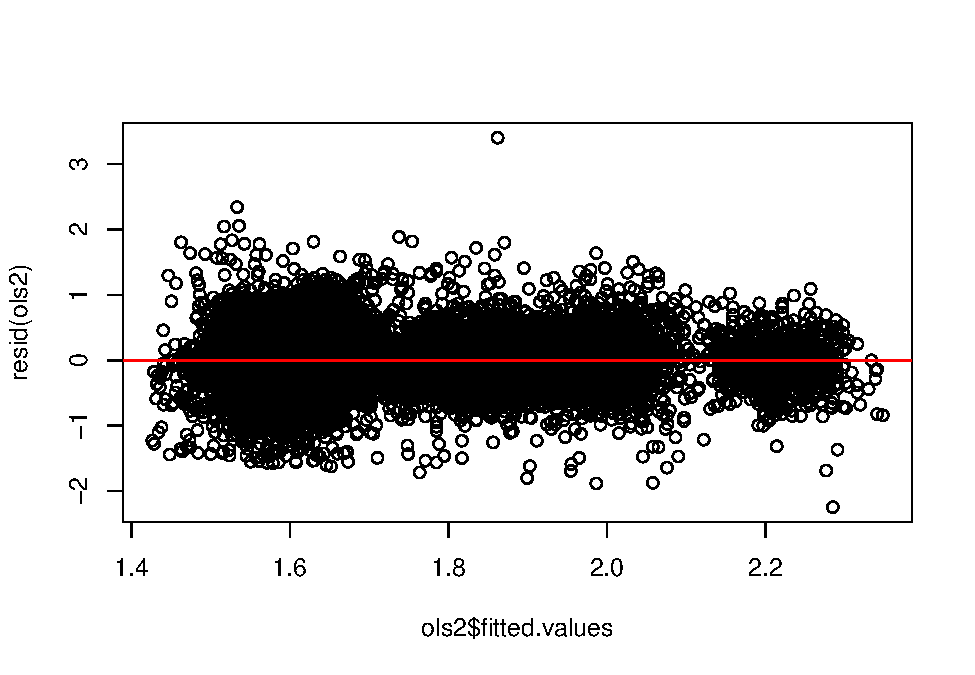
\includegraphics{Rintro2_files/figure-latex/unnamed-chunk-11-1.pdf}

\hypertarget{breusch-pagan-test}{%
\paragraph{Breusch-Pagan test}\label{breusch-pagan-test}}

\begin{verbatim}
## 
##  studentized Breusch-Pagan test
## 
## data:  ols2
## BP = 284.11, df = 4, p-value < 2.2e-16
\end{verbatim}

The results from the Breusch-Pagan test for the \texttt{ols2} model
suggest the presence of heteroscedasticity. The test statistic is
\(BP = 199.54\) with a degree of freedom (df) of 4. The low p-value,
effectively zero at \(p < 2.2e-16\), leads us to reject the null
hypothesis of homoscedasticity.

\hypertarget{robust-estimation}{%
\subsubsection{5.1.7. Robust estimation}\label{robust-estimation}}

\begin{Shaded}
\begin{Highlighting}[]
\NormalTok{robust\_ols2 }\OtherTok{\textless{}{-}} \FunctionTok{coeftest}\NormalTok{(ols2, }\AttributeTok{vcov. =} \FunctionTok{vcovHC}\NormalTok{(ols2, }\AttributeTok{type=}\StringTok{"HC1"}\NormalTok{))}
\FunctionTok{print}\NormalTok{(robust\_ols2)}
\end{Highlighting}
\end{Shaded}

\begin{verbatim}
## 
## t test of coefficients:
## 
##               Estimate Std. Error t value  Pr(>|t|)    
## (Intercept) 1.28788491 0.02783552 46.2677 < 2.2e-16 ***
## age         0.00713867 0.00058433 12.2168 < 2.2e-16 ***
## collgrad    0.37742427 0.00956496 39.4590 < 2.2e-16 ***
## union       0.21157873 0.00842208 25.1219 < 2.2e-16 ***
## hours       0.00249920 0.00053996  4.6285 3.718e-06 ***
## ---
## Signif. codes:  0 '***' 0.001 '**' 0.01 '*' 0.05 '.' 0.1 ' ' 1
\end{verbatim}

\begin{table}[!htbp] \centering 
  \caption{Comparison of OLS and Robust Regression Models} 
  \label{} 
\begin{tabular}{@{\extracolsep{5pt}}lcc} 
\\[-1.8ex]\hline 
\hline \\[-1.8ex] 
\\[-1.8ex] & ln\_wage &   \\ 
 & OLS & Robust OLS \\ 
\\[-1.8ex] & (1) & (2)\\ 
\hline \\[-1.8ex] 
 Constant & 1.288$^{***}$ & 1.288$^{***}$ \\ 
  & (0.023) & (0.028) \\ 
  & & \\ 
 age & 0.007$^{***}$ & 0.007$^{***}$ \\ 
  & (0.001) & (0.001) \\ 
  & & \\ 
 collgrad & 0.377$^{***}$ & 0.377$^{***}$ \\ 
  & (0.009) & (0.010) \\ 
  & & \\ 
 union & 0.212$^{***}$ & 0.212$^{***}$ \\ 
  & (0.009) & (0.008) \\ 
  & & \\ 
 hours & 0.002$^{***}$ & 0.002$^{***}$ \\ 
  & (0.0004) & (0.001) \\ 
  & & \\ 
\textit{N} & 13,452 &  \\ 
R$^{2}$ & 0.178 &  \\ 
Adjusted R$^{2}$ & 0.178 &  \\ 
Residual Std. Error & 0.417 (df = 13447) &  \\ 
F Statistic & 727.942$^{***}$ (df = 4; 13447) &  \\ 
\hline 
\hline \\[-1.8ex] 
\textit{Notes:} & \multicolumn{2}{r}{$^{***}$Significant at the 1 percent level.} \\ 
 & \multicolumn{2}{r}{$^{**}$Significant at the 5 percent level.} \\ 
 & \multicolumn{2}{r}{$^{*}$Significant at the 10 percent level.} \\ 
\end{tabular} 
\end{table}

\hypertarget{coefficient-interpretation-with-a-full-model-model-2}{%
\subsubsection{5.1.8. Coefficient interpretation with a full model
(Model 2)}\label{coefficient-interpretation-with-a-full-model-model-2}}

Given that our dependent variable is the natural logarithm of the
salary, the coefficients should be interpreted accordingly. For every
additional year in age, the salary is expected to increase by
approximately 0.7024557\%, holding all other factors constant. Being a
college graduate is associated with an estimated increase of about
45.7904309\% in the salary, compared to not being a college graduate.
Being a member of a union is associated with an approximate 23.6147885\%
increase in salary, holding everything else constant. All variables are
significant at the 1\% level.

\hypertarget{binary-choice-models}{%
\subsection{5.2. Binary choice models}\label{binary-choice-models}}

When the dependent variable is binary, ordinary least squares regression
is not suitable due to the non-continuous nature of the outcome
variable. Models such as Logit and Probit are specifically designed to
handle such binary outcomes. In our analysis, where we aim to understand
the probability of a worker being unionized, these models are
appropriate choices as they provide insights into the factors
influencing this binary decision.These models show the direction of the
relationship between independent variables and the dependent variable
but don't quantify the magnitude.

\begin{verbatim}
## 
## Call:
## glm(formula = union ~ ., family = binomial(link = "probit"), 
##     data = db_ols)
## 
## Coefficients:
##              Estimate Std. Error z value Pr(>|z|)    
## (Intercept) -2.467689   0.091163 -27.069   <2e-16 ***
## age         -0.001280   0.001970  -0.650    0.516    
## ln_wage      0.734203   0.030386  24.162   <2e-16 ***
## collgrad    -0.032086   0.032593  -0.984    0.325    
## hours        0.012740   0.001326   9.608   <2e-16 ***
## ---
## Signif. codes:  0 '***' 0.001 '**' 0.01 '*' 0.05 '.' 0.1 ' ' 1
## 
## (Dispersion parameter for binomial family taken to be 1)
## 
##     Null deviance: 14463  on 13451  degrees of freedom
## Residual deviance: 13640  on 13447  degrees of freedom
## AIC: 13650
## 
## Number of Fisher Scoring iterations: 4
\end{verbatim}

\% Table created by stargazer v.5.2.3 by Marek Hlavac, Social Policy
Institute. E-mail: marek.hlavac at gmail.com \% Date and time: ter, dez
05, 2023 - 21:45:30

\begin{table}[!htbp] \centering 
  \caption{Comparative Table of Logit and Probit Models} 
  \label{} 
\begin{tabular}{@{\extracolsep{5pt}}lcc} 
\\[-1.8ex]\hline 
\hline \\[-1.8ex] 
\\[-1.8ex] & \multicolumn{2}{c}{union} \\ 
\\[-1.8ex] & \textit{logistic} & \textit{probit} \\ 
\\[-1.8ex] & (1) & (2)\\ 
\hline \\[-1.8ex] 
 age & $-$0.003 & $-$0.001 \\ 
  & (0.003) & (0.002) \\ 
  & & \\ 
 ln\_wage & 1.253$^{***}$ & 0.734$^{***}$ \\ 
  & (0.053) & (0.030) \\ 
  & & \\ 
 collgrad & $-$0.053 & $-$0.032 \\ 
  & (0.055) & (0.033) \\ 
  & & \\ 
 hours & 0.022$^{***}$ & 0.013$^{***}$ \\ 
  & (0.002) & (0.001) \\ 
  & & \\ 
 Constant & $-$4.167$^{***}$ & $-$2.468$^{***}$ \\ 
  & (0.160) & (0.091) \\ 
  & & \\ 
\textit{N} & 13,452 & 13,452 \\ 
Log Likelihood & $-$6,825.528 & $-$6,820.092 \\ 
Akaike Inf. Crit. & 13,661.060 & 13,650.180 \\ 
\hline 
\hline \\[-1.8ex] 
\textit{Notes:} & \multicolumn{2}{r}{$^{***}$Significant at the 1 percent level.} \\ 
 & \multicolumn{2}{r}{$^{**}$Significant at the 5 percent level.} \\ 
 & \multicolumn{2}{r}{$^{*}$Significant at the 10 percent level.} \\ 
\end{tabular} 
\end{table}

\hypertarget{marginal-effects}{%
\subsubsection{5.2.1. Marginal effects}\label{marginal-effects}}

Marginal effects are crucial in non-linear models like Logit and Probit.
While the model's coefficients tell us about the direction of effects,
they don't show the actual change in probability for a one-unit change
in the predictor. Marginal effects provide this information, making it
easier to understand the real-world impact of each variable on the
outcome.

\hypertarget{marginal-effects---probit}{%
\paragraph{5.2.2. Marginal effects -
probit}\label{marginal-effects---probit}}

\begin{verbatim}
##    factor     AME     SE       z      p   lower  upper
##       age -0.0004 0.0006 -0.6497 0.5159 -0.0015 0.0007
##  collgrad -0.0091 0.0093 -0.9845 0.3249 -0.0273 0.0090
##     hours  0.0036 0.0004  9.6734 0.0000  0.0029 0.0044
##   ln_wage  0.2089 0.0082 25.4688 0.0000  0.1928 0.2250
\end{verbatim}

\hypertarget{marginal-effects---logit}{%
\paragraph{5.2.3. Marginal effects -
logit}\label{marginal-effects---logit}}

\begin{verbatim}
##    factor     AME     SE       z      p   lower  upper
##       age -0.0005 0.0006 -0.9483 0.3430 -0.0016 0.0006
##  collgrad -0.0088 0.0091 -0.9667 0.3337 -0.0266 0.0090
##     hours  0.0037 0.0004  9.6196 0.0000  0.0030 0.0045
##   ln_wage  0.2076 0.0083 25.1307 0.0000  0.1914 0.2238
\end{verbatim}

\hypertarget{summary-of-marginal-effects-for-logit-model-on-union-membership}{%
\paragraph{5.2.4. Summary of Marginal Effects for Logit Model on Union
Membership:}\label{summary-of-marginal-effects-for-logit-model-on-union-membership}}

\begin{itemize}
\item
  \textbf{Age:} A one-year increase in age is linked to a decrease in
  the likelihood of a worker being unionized by 0.05 percentage points.
  However, the effect is not statistically significant at the 5\% level
\item
  \textbf{College Graduation (collgrad):} Being a college graduate
  reduces the probability of being in a union by 0.88 percentage points.
  However, the effect is not statistically significant at the 5\% level
\item
  \textbf{Hours:} A one-unit increase in hours is associated with a 0.37
  percentage point increase in the likelihood of a worker being
  unionized.
\item
  \textbf{Log of Wage (ln\_wage):} A one-unit increase in the logarithm
  of wage is associated with a 20.76 percentage point increase in the
  likelihood of a worker being unionized.
\end{itemize}

\hypertarget{assessment}{%
\section{6 Assessment}\label{assessment}}

\hypertarget{problem-1-data-importing}{%
\subsection{Problem 1: Data Importing}\label{problem-1-data-importing}}

Import the ``card'' dataset.

\begin{Shaded}
\begin{Highlighting}[]
\NormalTok{card}\OtherTok{\textless{}{-}}\FunctionTok{as.data.frame}\NormalTok{(}\FunctionTok{read\_excel}\NormalTok{(}\StringTok{"card.xlsx"}\NormalTok{))}
\end{Highlighting}
\end{Shaded}

\hypertarget{problem-2-drop-the-missing-data}{%
\subsection{Problem 2: Drop the missing
data}\label{problem-2-drop-the-missing-data}}

\begin{Shaded}
\begin{Highlighting}[]
\CommentTok{\#}\RegionMarkerTok{BEGIN}\CommentTok{ SOLUTION}

\NormalTok{card\_no\_na }\OtherTok{\textless{}{-}} \FunctionTok{na.omit}\NormalTok{(card)}


\CommentTok{\#}\RegionMarkerTok{END}\CommentTok{ SOLUTION}
\end{Highlighting}
\end{Shaded}

\hypertarget{problem-3}{%
\subsection{Problem 3}\label{problem-3}}

Estimate a linear regression model that uses the log of the salary as
the dependent variable and IQ, married, age, educ, and the log of weight
as independent variables.

\begin{Shaded}
\begin{Highlighting}[]
\CommentTok{\#}\RegionMarkerTok{BEGIN}\CommentTok{ SOLUTION}


\CommentTok{\#}\RegionMarkerTok{END}\CommentTok{ SOLUTION}
\end{Highlighting}
\end{Shaded}

\hypertarget{problem-4}{%
\subsection{Problem 4:}\label{problem-4}}

Which variables are the most important in the model? Explain

\begin{Shaded}
\begin{Highlighting}[]
\CommentTok{\#}\RegionMarkerTok{BEGIN}\CommentTok{ SOLUTION}


\CommentTok{\#}\RegionMarkerTok{END}\CommentTok{ SOLUTION}
\end{Highlighting}
\end{Shaded}

\hypertarget{problem-5-what-can-you-conclude-regarding-homoscedasticity}{%
\subsection{Problem 5: What can you conclude regarding
homoscedasticity?}\label{problem-5-what-can-you-conclude-regarding-homoscedasticity}}

\begin{Shaded}
\begin{Highlighting}[]
\CommentTok{\#}\RegionMarkerTok{BEGIN}\CommentTok{ SOLUTION}


\CommentTok{\#}\RegionMarkerTok{END}\CommentTok{ SOLUTION}
\end{Highlighting}
\end{Shaded}

\hypertarget{problem-6}{%
\subsection{Problem 6:}\label{problem-6}}

Interpret the coefficients of the variables

\begin{Shaded}
\begin{Highlighting}[]
\CommentTok{\#}\RegionMarkerTok{BEGIN}\CommentTok{ SOLUTION}

\CommentTok{\#}\RegionMarkerTok{END}\CommentTok{ SOLUTION}
\end{Highlighting}
\end{Shaded}

\hypertarget{problem-7}{%
\subsection{Problem 7:}\label{problem-7}}

Create a binary variable that takes the value 1 if the salary is above
the average and 0 otherwise

\begin{Shaded}
\begin{Highlighting}[]
\NormalTok{average\_wage }\OtherTok{\textless{}{-}} \FunctionTok{mean}\NormalTok{(card\_no\_na}\SpecialCharTok{$}\NormalTok{wage)}

\CommentTok{\# Create a binary variable (high wage): 1 if wage is above average, 0 otherwise}
\NormalTok{card\_no\_na }\OtherTok{\textless{}{-}}\NormalTok{ card\_no\_na }\SpecialCharTok{\%\textgreater{}\%}
  \FunctionTok{mutate}\NormalTok{(}\AttributeTok{high\_wage =} \FunctionTok{ifelse}\NormalTok{(wage }\SpecialCharTok{\textgreater{}}\NormalTok{ average\_wage, }\DecValTok{1}\NormalTok{, }\DecValTok{0}\NormalTok{))}
\end{Highlighting}
\end{Shaded}

\hypertarget{problem-8}{%
\subsection{Problem 8:}\label{problem-8}}

Estimate a logit model to explain the probability of an individual
having a salary above the average, using the same independent variables
as in the linear regression mode.

\begin{Shaded}
\begin{Highlighting}[]
\CommentTok{\#}\RegionMarkerTok{BEGIN}\CommentTok{ SOLUTION}

\CommentTok{\#}\RegionMarkerTok{END}\CommentTok{ SOLUTION}
\end{Highlighting}
\end{Shaded}

\hypertarget{problem-9}{%
\subsection{Problem 9:}\label{problem-9}}

Discuss how the independent variables are positively/negatively related
to the probability of the salary being above the average.

\begin{Shaded}
\begin{Highlighting}[]
\CommentTok{\#}\RegionMarkerTok{BEGIN}\CommentTok{ SOLUTION}

\CommentTok{\#}\RegionMarkerTok{END}\CommentTok{ SOLUTION}
\end{Highlighting}
\end{Shaded}

\hypertarget{problem-10}{%
\subsection{Problem 10:}\label{problem-10}}

Compute the marginal effects of the logit model

\begin{Shaded}
\begin{Highlighting}[]
\CommentTok{\#}\RegionMarkerTok{BEGIN}\CommentTok{ SOLUTION}

\CommentTok{\#}\RegionMarkerTok{END}\CommentTok{ SOLUTION}
\end{Highlighting}
\end{Shaded}


\end{document}
